%\todo{2S - сюда нужно вставить переведенные текст с картинками materials\/jmb\_2016\/paper.docx, картинки нужно засунуть в гугл Draw (папка p2) - там перевести наложив поверх английского текста русский. Ссылки на литературу уже загружены в зотеро (если вдруг чего-то нет, нужно написать мне). Все заголовки начинать с уровне subsection и далее}

    При формировании нуклеосом октамер гистоновых белков организует около 200 пар оснований ДНК в два суперспиральных витка. Хотя статическая структура коровой частицы нуклеосомы была разрешена, детали динамических взаимодействий между гистонами и ДНК остаются не совсем понятными. Для изучения данного вопроса мы провели длительное равновесное моделирование молекулярной динамики нуклеосом, включая линкерные сегменты ДНК и полноразмерные гистоны, в явном растворителе в атомистическом приближении. Впервые мы смогли идентифицировать и охарактеризовать перестройки в нуклеосомах на микросекундном масштабе времени, изучить связь между конформацией гистоновых хвостов и геометрией ДНК. Мы обнаружили, что определенные конформации гистонового хвоста способствовали выпячиванию ДНК вблизи участков ее входа/выхода в/из нуклеосомы, что приводило к образованию дефектов кручения внутри ДНК. Мы охарактеризовали динамику гистоновых хвостов при их конденсации на нуклеосомальной и линкерной ДНК и показали, что хвосты могут принимать конформационно ограниченные позиции из-за вставки  лизинов и аргининов в малые бороздки ДНК. Потенциально, эти явления влияют на доступность посттрансляционно модифицированных остатков гистонов, которые служат важными сайтами для эпигенетических меток (например, в H3K9, H3K27, H4K16). Предполагается, что взаимодействия гистоновых хвостов с коровой и линкерной ДНК модулируют процессы взаимодействия белков хроматина с гистонами, модификации хвостов и связывания эффекторных белков. В данном разделе мы обсуждаем влияние наблюдаемых явлений на функцию нуклеосом и сравниваем наши результаты с различными экспериментальными исследованиями.

\subsection{Введение}
    Нуклеосомы - это элементарные единицы компактизации хроматина в геномах эукариот, расположенные через каждые 200 $\pm$ 40 п.н. вдоль ДНК \cite{mcghee_nucleosome_1980}. Основным источником информации об атомистической структуре нуклеосомы являются рентгеновские исследования коровых частиц нуклеосом (NCP) (см. обзор \cite{dechassa_nucleosomes_2011}), которые неизменно разрешают очень похожие структуры гистонов и ДНК независимо от вариантов последовательности гистонов, мутаций, посттрансляционные модификации, последовательности ДНК или присутствия белков, связывающих нуклеосомы, пептидов или химических агентов. Например, суперпозиция различных структур нуклеосом с использованием алгоритма VAST+ \cite{madej_mmdb_2014} показала очень небольшие вариации в среднеквадратичном отклонении (RMSD) около 1 \AA для выровненных глобулярных частей гистоновых областей. Консенсусная структура NCP формируется путем наматывания $\sim$ 145-147 п.н. коровой ДНК в $\sim$ 1,7 левых сверхспиральных витка вокруг октамера, состоящего из четырех типов коровых гистонов (H3, H4, H2A, H2B) \cite{marino-ramirez_histone_2011}. Структура NCP характеризуется наличием диадной оси - оси псведосимметрии второго порядка, сильно изогнутой структурой ДНК \cite{tolstorukov_novel_2007} и высоким положительным зарядом октамера гистонов \cite{fenley_charge_2010}. Кроме того, он включает большое количество молекул воды, проникающих в структуру нуклеосомы \cite{davey_solvent_2002}, а также длинные гистоновые хвосты, выступающие из ядра нуклеосомы и обеспечивающие множество сайтов для посттрансляционных модификаций (ПТМ).

    С другой стороны, решающая роль нуклеосом в функционировании хроматина (включая тонкую регуляцию экспрессии генов, репликацию ДНК, репарацию и наследование, опосредованные эпигенетическими механизмами \cite{henikoff_nucleosome_2008,petty_balancing_2013}) зависит от их динамической природы и конформационных переходов. Действительно, многие биофизические (FRET, эксперименты с одномолекулярными пинцетами и другие, рассмотренные в \cite{choy_structural_2012}) и биохимические эксперименты (анализ связывания факторов транскрипции \cite{li_rapid_2005}, химическая сшивка \cite{lee_n-terminal_1997}, анализ методом ChIP-exo  \cite{rhee_subnucleosomal_2014}) предполагают, что нуклеосомы демонстрируют существенный конформационный полиморфизм как на локальном (конформация ДНК и гистоновых хвостов внутри нуклеосомы), так и на глобальном (потеря гистонов, субнуклеосомные частицы и т. д.) масштабах, которые, в свою очередь, могут быть результатом равновесных тепловых флуктуаций или могут быть активно индуцированы внешними силами внутри клетки.
    
    Были предложены различные функционально значимые моды динамики нуклеосом, которые включают дыхание/разворачивание/раскрытие ДНК, расщепление нуклеосом \cite{zlatanova_nucleosome_2009}, а также скольжение нуклеосом \cite{mueller-planitz_nucleosome_2013}, раскрытие или потерю димера H2A-H2B \cite{shaytan_nucleosome_2015}. В то же время, различные конформационные перестройки гистоновых хвостов необходимы для внутри- и межнуклеосомных взаимодействий \cite{pepenella_intra-_2014}, для множественных взаимодействий с ремоделерами хроматина \cite{hwang_histone_2014,racki_histone_2014}, гетерохроматиновыми белками \cite{wang_heterochromatin_2013} и со многими эффекторными белками, которые содержат домены, связывающие модификации гистонов \cite{rando_combinatorial_2012}. Тем не менее, взгляду на нуклеосомы как на динамические объекты \cite{zlatanova_nucleosome_2009} все еще не хватает понимания деталей на атомистическом уровне.

    Чтобы попытаться сгладить этот очевидный пробел в нашем понимании динамики и функций нуклеосом, уже были предприняты значительные усилия в области моделирования, включая моделирование молекулярной динамики (МД) на атомистическом уровне \cite{biswas_atomistic_2013} и моделирование в крупнозернистом приближении \cite{arya_role_2006,collepardo-guevara_chromatin_2014}. Однако из-за значительного размера нуклеосомы по стандартам атомистического моделирования и чрезвычайно долгих временных масштабов ее функциональной динамики в предыдущих исследованиях приходилось прибегать либо к крупнозернистому моделированию без атомистических деталей, либо к полностью атомному моделированию без явных молекул растворителя \cite{erler_role_2014}. Полноатомное моделирование проводилось на временах не превышающих нескольких сотен наносекунд \cite{materese_counterion_2009,ruscio_computational_2006}. Однако мы знаем, что изменения в атомных взаимодействиях могут иметь глубокие функциональные последствия для нуклеосом. Например, посттрансляционные модификации могут изменять внутри- и межнуклеосомные взаимодействия или обеспечивать множественные сайты связывания для так называемых эффекторных белков \cite{ruthenburg_multivalent_2007}, даже однократное ацетилирование H4K16 может запускать разворачивание хроматиновых волокон \cite{dorigo_chromatin_2003,norouzi_topological_2015-1}.

    В работе, изложенной в данном разделе, концептуальный прогресс состоит в том, чтобы использовать наиболее надежный подход моделирования методом МД с явным  растворителем для всех атомов  и расширить этот подход на значительно более длительную микросекундную шкалу времени. Микросекундное моделирование, а также модели нуклеосом с реалистичными сегментами ДНК-линкера и многочисленные сравнительные модели позволили нам получить представление о функционально значимых перестройках в нуклеосомах, включая связь между конформациями гистоновых хвостов и геометрией ДНК. Хотя многие функционально релевантные движения могут происходить в гораздо более длительных временных масштабах \cite{choy_structural_2012}, несколько недавних исследований ЯМР показали, что гистоновые хвосты демонстрируют субмикросекундную динамику, что дает возможность сравнить наши расчетные результаты с экспериментальными данными \cite{kato_characterization_2009,zhou_histone_2012,gao_histone_2013}.

    В этом исследовании мы обнаружили, что определенные конформации гистонового хвоста способствуют выпячиванию ДНК возле мест входа/выхода ДНК в нуклеосоме, образованию дефектов кручения внутри ДНК и перестройке взаимодействий гистонов с ДНК в нуклеосомном коре. Мы охарактеризовали динамику гистоновых хвостов при их конденсации на коровой и линкерной ДНК на атомистическом уровне и показали, что они могут принимать конформационно ограниченные положения, сопровождаемые вставкой определенных ``закрепляющих'' лизинов и аргининов в малые бороздки ДНК. Мы предполагаем, что эти процессы влияют на доступность посттрансляционно модифицированных остатков гистонов, которые служат важными эпигенетическими метками (например, H3K9, H3K27, H4K16), а взаимодействия с коровой и особенно линкерной ДНК (для хвоста H3) могут модулировать доступность различных сайтов на гистоновых хвостах для связывания эффекторными белками.

\subsection{Результаты}

\subsubsection{Обзор исследованных моделей}
В нашем исследовании мы использовали несколько систем для моделирования, в том числе специально сконструированную полную нуклеосомную систему с линкерными сегментами ДНК по 20 п.н., фланкирующих коровую частицу с каждой стороны (модель FN) (Рис. \ref{fig:p2_2_f1}а), минималистичную модель коровой частицы с усеченными гистоновыми хвостами (NCPm модель) и набор вспомогательных систем с различными условиями моделирования (подробности см. в таблице \ref{tbl:p2:jmb_t1}). Ниже мы в основном сосредотачиваемся на результатах, полученных для полной нуклеосомной системы, для которой были выполнены обширные микросекундные расчеты. Мы допускаем, что динамика нуклеосом происходит в нескольких временных масштабах, а функционально значимые конформационные переходы часто превышают масштаб времени в одну микросекунду. Наше моделирование ограничивалось исследованием конформационных ансамблей вокруг определенных локальных квазиравновесных состояний в микросекундной шкале времени. Поэтому, интерпретируя результаты нашего моделирования, проверяли наши выводы, выполняя несколько вспомогательных расчетов. При обсуждении результатов ниже мы ссылаемся на ключевые структурные элементы гистоновых последовательностей и нуклеосом, как показано на рисунке \ref{fig:p2_2_f2} (см. Также раздел ``Название элементов структуры нуклеосом'' ниже).


\begin{table}[p]
\caption{Исследованные в моделировании системы и их параметры}
	\label{tbl:p2:jmb_t1}	
	\begin{tabularx}{\textwidth} { 
  | >{\raggedright\arraybackslash}X 
  | >{\centering\arraybackslash}X 
  | >{\raggedleft\arraybackslash}X 
  | >{\raggedleft\arraybackslash}X 
  | >{\raggedleft\arraybackslash}X 
  | >{\raggedleft\arraybackslash}X |}
  \hline
Название & Описание & Количество атомов, тыс. & Эффект. концентрация соли, мМ & Размер ячейки, \AA & Время моделирования, нс\\
	\hline

FN & Система с линкерной ДНК и гистоновыми хвостами & 366,8 & $\sim$185 & 162х197х113 & 1000 \\
\hline
FN1M & То же, что и не FN, но в высокой концентрации соли & 366,8 & $\sim$1100 & 161х196х112 & 1000 \\
\hline
FNbb & То же, что и не FN, но в большей ячейке & 3200 & $\sim$160 & 322х358х274 & 1000 \\
\hline
FNnt & То же, что и не FN, но с ацетильными и N-метил группами на концах гистонов& 366,8 & $\sim$185 & 162х197х113 & 1000 \\
\hline
NCPm & Cистема, без линкерной ДНК и хвостов гистонов & 310,3 & $\sim$200 & 145х141х101 & 1000 \\
\hline

\end{tabularx}
	 
\end{table}

\begin{figure} [H]
    \centering
    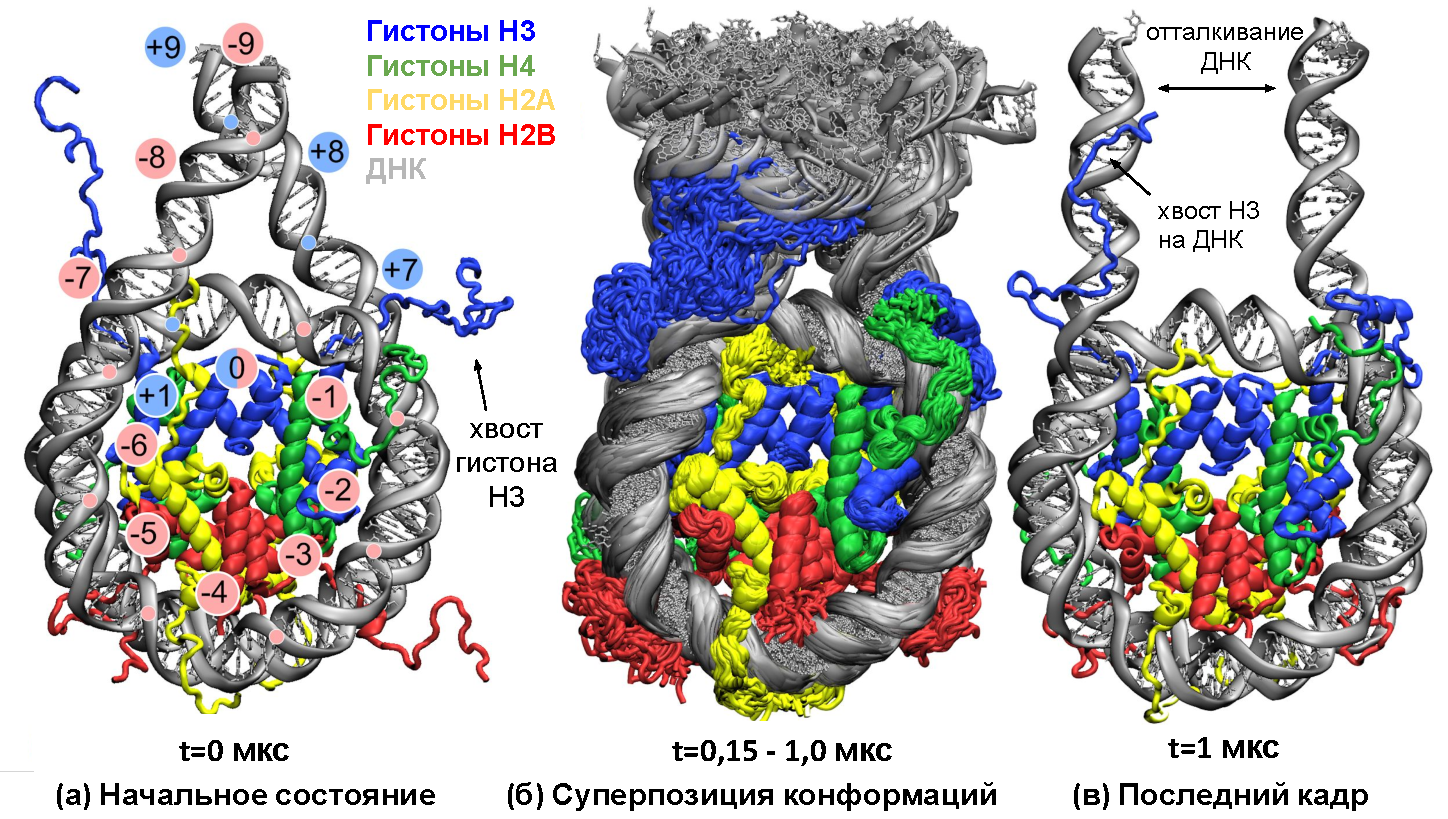
\includegraphics[width=\textwidth]{images/p2/jmb/part2_2_f1.pdf}
    \caption[Обзор структуры и динамики модели полной нуклеосомы (FN)]{Обзор структуры и динамики модели полной нуклеосомы (FN): (a) Исходная структура модели FN, (б) наложенные конформации из последних 75 \% кадров расчетной траектории, (в) последний кадр после 1 мкс, обратите внимание на различные формы N-концевых хвостов H3 с обеих сторон.}
    \label{fig:p2_2_f1}
\end{figure}

\begin{figure} [H]
    \centering
    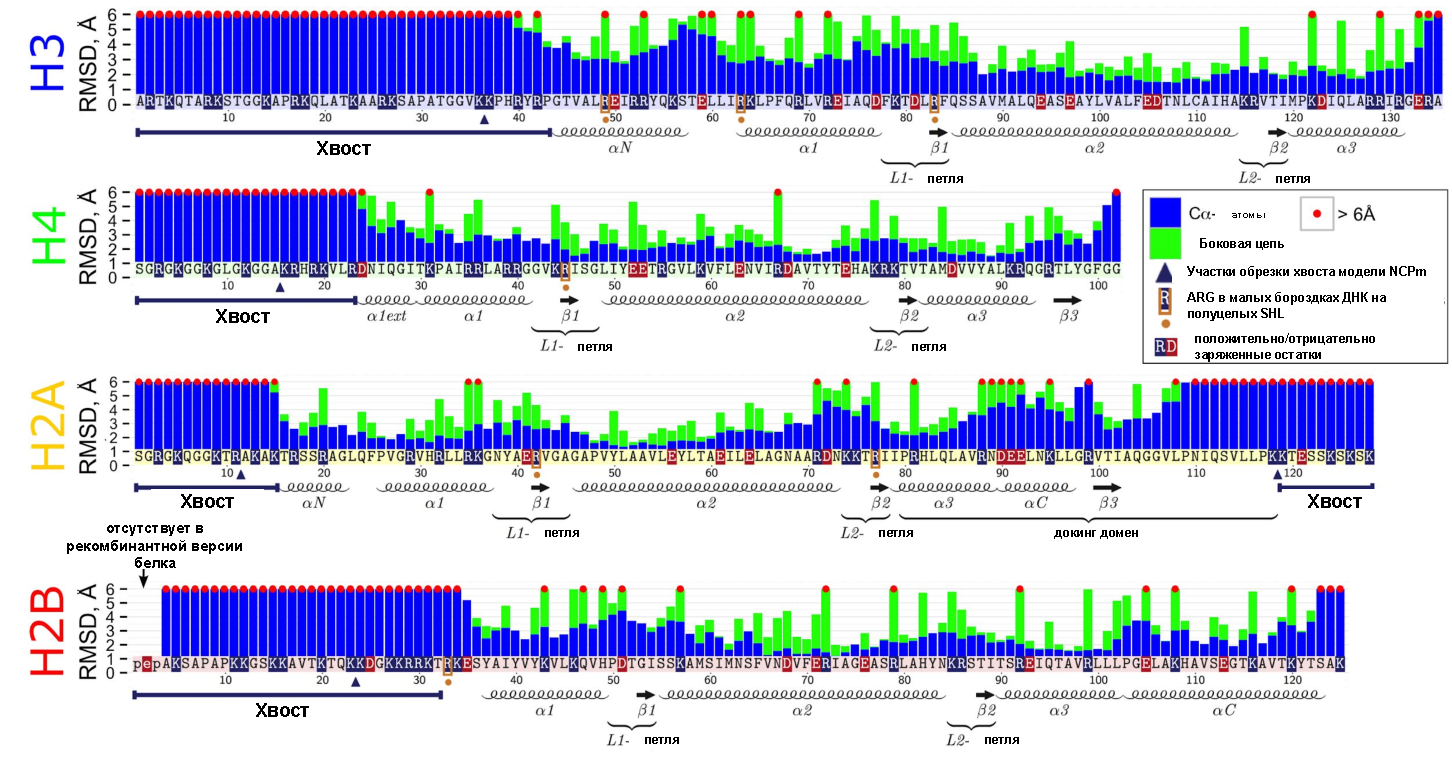
\includegraphics[width=\textwidth]{images/p2/jmb/part2_2_f2.pdf}
    \caption[Максимальные наблюдаемые среднеквадратичные отклонения отдельных аминокислот гистонов 
    в МД моделировании]{Максимальные наблюдаемые среднеквадратичные отклонения отдельных 
    аминокислот (C$\alpha$-атомы - синие столбцы, атомы боковой цепи - зеленые столбцы) во время
     моделирования относительно их положения в исходной рентгеновской структуре. 
     Значения, превышающие 6\AA, усекаются при этом значении и отмечаются красной точкой над столбцом.
      Аннотации структурных элементов гистонов приведены под столбиками.}
    \label{fig:p2_2_f2}
\end{figure}



\subsubsection{Конформационная стабильность и пластичность гистонов и ДНК}

    В соответствии с предыдущими экспериментальными исследованиями, наше моделирование подтвердило общую стабильность ядра нуклеосомы в отношении диссоциации компонентов нуклеосомы или крупномасштабного развертывания ДНК (см. Обзор динамики на рисунке \ref{fig:p2_2_f1}). В целом, RMSD центральной области гистонов оставалось в среднем в пределах 1,5\AA от кристаллографических положений для всех изученных моделей. Это было верно даже для минималистичной системы NCPm с усеченными гистоновыми хвостами. Таким образом, предполагается, что нуклеосомы имеют достаточный запас стабильности в отношении усечения гистоновых хвостов на микросекундных временах. Однако подробный анализ конформационной динамики, представленный ниже, предоставил новое понимание конформационной гибкости нуклеосом и выявил конформационные перестройки внутри гистонового ядра, гистоновых хвостов, ядра ДНК и линкерных областей, которые происходят в микросекундной шкале времени.

    Чтобы предоставить подробную картину динамики гистонов, мы изобразили максимальные отклонения позиций атомов, наблюдаемые в ходе динамики, от положений в кристаллической структуре (Рис. \ref{fig:p2_2_f2}). Как можно видеть на рисунке \ref{fig:p2_2_f2}, относительно большие конформационные изменения более чем на 6\AA наблюдались для атомов остова всех хвостов гистонов, даже некоторые части гистоновых фолдов демонстрируют высокое RMSD. Хотя, как показывает анализ кристаллических структур, докинг домен H2A (docking domain) образует тесные контакты с тетрамером $(H3-H4)_2$ \cite{suto_crystal_2000}, мы продемонстрировали существенные конформационные изменения для С-концевой части этого домена относительно исходной кристаллической структуры. Конформационные флуктуации остова белковой цепи часто сопровождались переориентацией боковых цепей аминокислотных остатков. Например, изменения в $\alpha$C-спирали докинг-домена сопровождались временным образованием новых солевых мостиков между H2A R88 и R99, фланкирующими эту спираль, и H3 E105, D106. Наблюдаемая пластичность докинг-домена будет влиять на его функции в качестве партнера по связыванию белков хроматина. В частности, недавно было показано, что шаперон ANP32E может быть ответственным за встраивание гистона H2A.Z в нуклеосому. ANP32E может связываться с $\alpha$C-спиральной областью докинг-домена H2A.Z \cite{obri_anp32e_2014}, которая в нуклеосоме структурно очень похожа на каноническую $\alpha$C-спираль H2A. Связывание гистона с ANP32E стерически несовместимо с полной структурой нуклеосомы и может запускать разборку и вытеснение нуклеосом, когда гибкая область ANP32E вставляется в кор нуклеосомы. Последний процесс не очень хорошо изучен, однако повышенная конформационная гибкость в этой области, наблюдаемая в нашем исследовании, указывает на возможные механизмы этого процесса. Интересно, что Biswas et al. в более ранних работах по МД моделированию нуклеосом показали потенциальную связь между усечением гистоновых хвостов H3 и конформациями боковых цепей H2A R81 и R88 \cite{biswas_role_2011}. Визуальное исследование траекторий динамики наших систем показывает, что, хотя боковая цепь H2A R88 очень гибкая в микросекундном масштабе времени, боковая цепь H2A R81 в основном заблокирована в своей кристаллографической ориентации и иногда перескакивает в положение, направленное в сторону от октамера гистонов. В последнем положении боковая цепь может находиться сотни наносекунд.

    Кроме того, значительные смещения остова полипептидной цепи (более 3\AA) и боковых цепей (более 6\AA) наблюдались в центральных областях других гистонов, включая H3 $\alpha$N-спираль, H3 $\alpha$1-спираль, сайт связывания L1-L2 димера H2A-H2B и H2B $\alpha$C-спираль) (Рис. \ref{fig:p2_2_f2}). Как уже упоминалось, даже если остов белка не демонстрирует больших отклонений от кристаллографических положений, все же могут происходить значительные изменения конформеров боковых цепей. Фактически, все аминокислоты, кроме одной, с наблюдаемой переориентацией боковой цепи более 6\AA, принадлежали заряженным остаткам. Эти переориентации часто включают разрушение и образование новых солевых мостиков внутри гистонового ядра. Изменения в модели NCPm показали аналогичные закономерности.


    Анализ конформационной динамики коровой и линкерной ДНК показал, что ДНК оставалась в среднем в пределах 4\AA (5 \AA для модели NCPm) от своих кристаллографических положений, измеренных с помощью RMSD атомов N1 и N9 азотистых оснований. Кроме того, фосфатный остов ДНК характеризуется периодическим профилем средних флуктуации (RMSF): участки остова ДНК, контактирующие с гистонами, проявляли значительно меньшие колебания по сравнению с теми, которые были обращены в раствор. С другой стороны, линкерные сегменты ДНК в нашем моделировании явно демонстрировали гораздо более сильные колебания, чем коровые участки ДНК (Рис. \ref{fig:p2_2_f1}б,в), что согласуется с известными данными \cite{pachov_structure_2011}. Глобальная конформация ДНК была дополнительно изучена с помощью 2D-проекций многоугольников, соединяющих центры пар оснований ДНК в нуклеосомной суперспиральной системе отсчета (см. Рис. \ref{fig:p2_2_f3}). Позиционные колебания линкерных сегментов ДНК охватывают частично перекрывающиеся конусообразные области в пространстве с угловым размахом около $\pm$45 градусов в обеих проекциях. Никаких существенных корреляций в позиционных колебаниях линкеров ДНК обнаружено не было. Средние положения, принятые для линкерных цепей ДНК в MD, были дальше друг от друга по сравнению с их исходными положениями, которые соответствовали прямому продолжению концов коровой ДНК (Рис. \ref{fig:p2_2_f3}а). Моделирование той же системы, но в солевом растворе с высоким содержанием 1 М (система FN1M) ясно показало, что два линкера ДНК приближаются друг к другу и даже большую часть времени взаимодействуют своими концами. Предполагаем, что скрининг электростатических взаимодействий значительно повлиял на угол входа/выхода ДНК. Интересно, что более ранние экспериментальные измерения расстояний между линкерами с помощью FRET показали, что расстояние монотонно уменьшается с увеличением концентрации соли \cite{toth_chromatin_2006}.

    Первостепенным вопросом динамики нуклеосом является амплитуда, временная шкала и механизмы отворачивания/дыхания ДНК, разворачивания или открытия поверхности октамера гистонов, что, как полагают, имеет решающее значение для доступности ДНК и связывания факторов транскрипции \cite{li_rapid_2005,mirny_nucleosome-mediated_2010}. К сожалению, на сегодняшний день нет полной картины, поскольку разные экспериментальные установки, интерпретация и терминология часто поддерживают разные взгляды на эту проблему \cite{choy_structural_2012,zlatanova_nucleosome_2009}. В этом исследовании мы не наблюдали крупномасштабного разворачивания или раскрытия коровой ДНК ни в системах FN, ни в системах NCPm. Такое разворачивание, если оно произойдет, обнажит достаточно частей ДНК для распознавания факторами транскрипции. Наши результаты согласуются с экспериментальными оценками временных масштабов событий разворачивания, которые лежат в субсекундном диапазоне \cite{li_rapid_2005,tomschik_nucleosome_2009}. Однако, если мы рассмотрим более умеренные колебания концов коровой ДНК вместе с линкерной ДНК (часто называемые ``дыханием ДНК''), такие процессы могут происходить в более коротких временных масштабах \cite{gansen_nucleosome_2009}. Например, недавние измерения FRET расстояний между двумя красителями, расположенными симметрично на обоих сегментах линкерной ДНК на расстоянии 5 п.н. от сайтов входа / выхода ДНК, показали две разные конформации с характерными расстояниями между двумя красителями $\sim$4,5 нм и $\sim$6,5 нм (амплитуда около 2 нм), в предположении  модели с двумя состояниями \cite{nurse_clipping_2013}. В нашем моделировании расстояние между центрами пар оснований соответствующих позиций линкеров ДНК варьировалось от 4,5 нм до 6,8 нм (см. Рис. \ref{fig:p2_2_f3}) (со средним значением 5,6 нм и RMSF 0,4 нм), показывая, что эти диапазоны расстояний находятся в пределах досягаемости быстрых субмикросекундных колебаний. Кроме того, мы наблюдали асимметрию в средних конформациях ДНК двух линкеров, а также в их отклонениях от исходной кристаллической структуры (обозначенной стрелками на рисунке \ref{fig:p2_2_f3}). Интересно, что если мы предположим, что наблюдаемые асимметрии соответствуют двум различным стабильным конформационным состояниям ДНК в нуклеосоме, переход между этими состояниями может уже объяснить изменение положения ДНК в  0,5 нм на расстоянии 5 п.н. от входа/выхода. Однако мы признаем, что методология для точного сравнения различных конформационных переходов, наблюдаемых при моделировании, и результатов измерений FRET все еще требует разработки и проверки: как недавно было отмечено Ленцем и др., флуктуация формы ДНК в нуклеосоме может размывать сигналы FRET от промежуточных конформационных состояний ДНК в нуклеосоме \cite{lenz_influence_2015}.

    В следующих разделах мы продемонстрируем, что эти конформационные асимметрии ДНК следствие асимметричной конденсацией гистоновых хвостов. Хотя мы находим, что время, необходимое для переключения между различными конформациями гистоновых хвостов, явно превышает микросекундную шкалу времени, мы предполагаем, что динамика ДНК в микросекундной шкале времени определяется взаимодействиями между гистоновыми хвостами и ДНК, которые, в свою очередь, могут влиять на конформацию ДНК на гораздо более длительных временах.
    %корявый перевод получился последнего абзаца, не понимаю как на русском правильно написать

\begin{figure} [H]
    \centering
    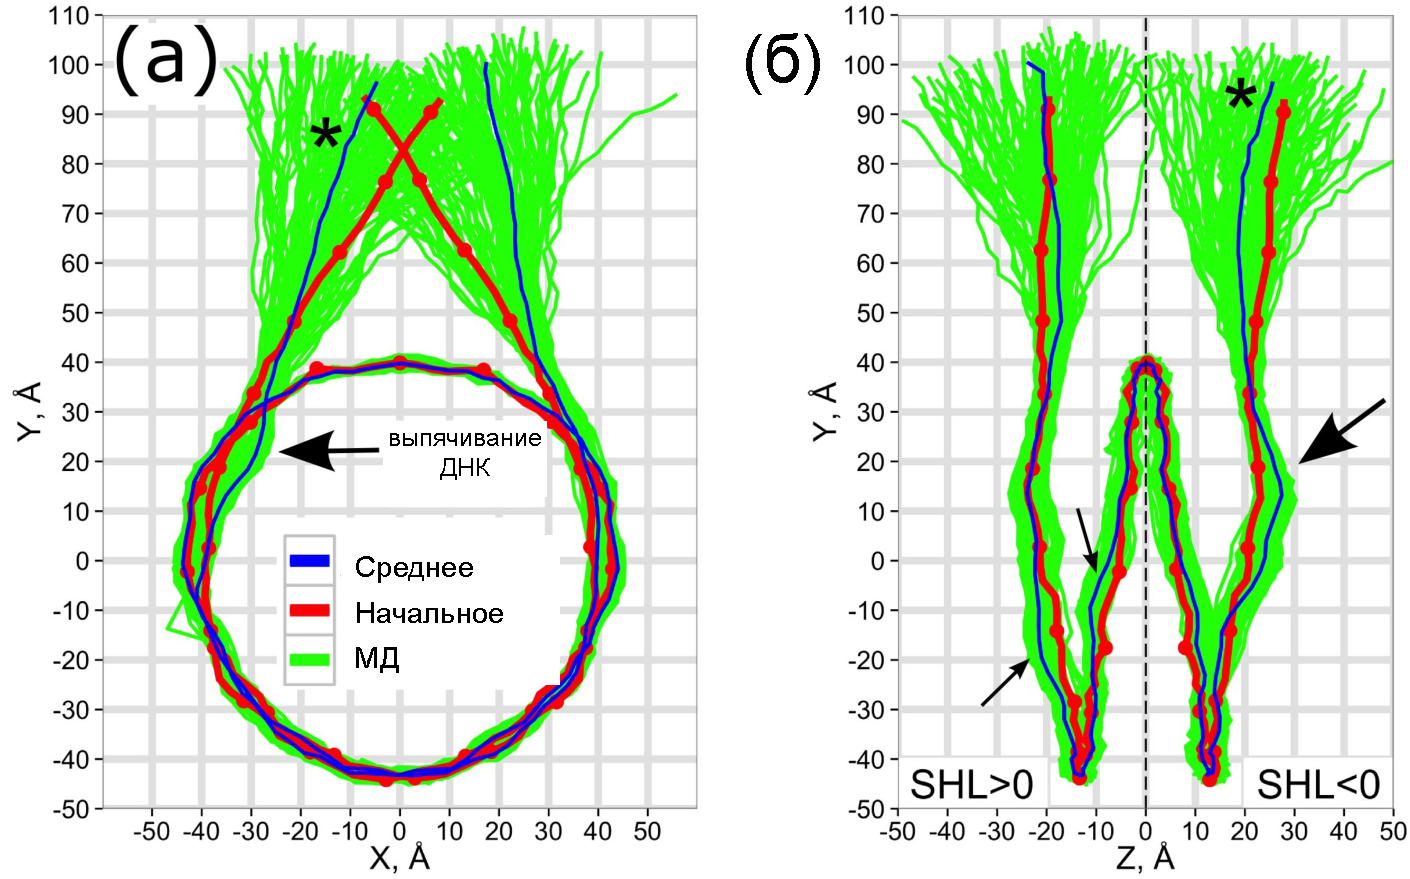
\includegraphics[width=\textwidth]{images/p2/jmb/part2_2_f3.pdf}
    \caption[Конформационный ансамбль ДНК в нуклеосоме]{Конформационный ансамбль ДНК в нуклеосоме, (а) - передняя и (б) - боковые проекции. Красными точками отмечены целые и полуцелые значения суперспирального положения (SHL) вдоль исходной конформации, звездочкой отмечен один линкерный сегмент ДНК на обоих рисунках. Стрелки указывают максимальные отклонения между исходной и средней конформациями в МД.}
    \label{fig:p2_2_f3}
\end{figure}

\subsubsection{Быстрая конденсация гистоновых хвостов на коровой и линкерной ДНК}
    Положительно заряженные гистоновые хвосты были тщательно изучены как экспериментально, так и с помощью методов моделирования. Известно, что межнуклеосомные взаимодействия опосредуются хвостами и играют важную роль в уплотнении хроматина. В этой работе мы охарактеризовали динамику взаимодействий между гистонами и ДНК на атомном уровне и обнаружили, что в среднем 60\% всех контактов были обеспечены взаимодействиями ДНК с участками гистонового хвоста. Хвосты гистонов, которые в исходной модели выступали в объем растворителя (в основном хвосты H3, Рис. \ref{fig:p2_2_f1}а), быстро адсорбировались на ДНК в течение первых 20 нс моделирования. От 50 до 90\% всех аминокислот в этих хвостовых областях имели прямые или опосредованные водой взаимодействия с коровой или линкерной ДНК в течение 1 мкс моделирования (Рис. \ref{fig:p2_2_f4}). Какого-либо существенного скопления контактов к началу или концу хвостов мы не наблюдали. Предыдущие полноатомные МД расчеты нуклеосомных частиц также указали на значительную ассоциацию гистоновых хвостов с коровой ДНК на временном масштабе 100 нс \cite{erler_role_2014,biswas_role_2011,roccatano_structural_2007}. Однако были высказаны определенные опасения по поводу коротких временных масштабов моделирования, а также артефактов, возникающих из-за периодических граничных условий и решеточных методов суммирования электростатических взаимодействий. Чтобы решить последнюю проблему, мы выполнили моделирование на протяжении 80 нс в большой ячейке (система FNbb), размер которой должен минимизировать потенциальные неблагоприятные эффекты периодических граничных условий. Моделирование FNbb подтвердило предпочтительную ассоциацию гистоновых хвостов с ДНК и быструю конденсацию длинных N-концевых хвостов H3. Таким образом, мы снимаем ранее высказанные опасения и показываем, что конденсация гистонового хвоста не является артефактом конкретных методов, используемых в МД-моделировании.

    Несколько исследований малоуглового рассеяния рентгеновских лучей (SAXS) касались вопроса о том, выступают ли гистоновые хвосты из ядра нуклеосомы в раствор или связаны с ДНК с физиологической ионной силой. Сообщалось о значительном увеличении максимального диаметра нуклеосом при повышении концентрации одновалентной соли с 10 мМ до физиологических концентраций и выше \cite{mangenot_salt-induced_2002}. Этот результат был приписан процессу диссоциации гистоновых хвостов от кора нуклеосомы. Однако Ян и др. \cite{yang_biophysical_2011} указали, что сопоставимое увеличение диаметра можно объяснить конформационными изменениями нуклеосом, включая разворачивание ДНК. Наши результаты подтверждают модель, в которой гистоновые хвосты прикреплены к коровой или линкерной ДНК большую часть времени в этой временной шкале. Если по какой-то причине хвосты оторвались, характерное время их присоединения должно составить около нескольких десятков наносекунд, о чем свидетельствует их быстрая конденсация (Рис. \ref{fig:p2_2_f4}). Наши теоретические оценки радиусов гирации предполагают, что и гистоновые хвосты, и линкерная ДНК вносят вклад в увеличение радиусов гирации.

    Чтобы дополнительно выяснить влияние концентрации соли на поведение хвоста, мы выполнили моделирование при чрезвычайно высокой концентрации соли 1M (модель FN1M). Хотя известно, что октамерная форма нуклеосом нестабильна при такой концентрации соли \cite{wilhelm_reconstitution_1978}, мы не наблюдали никакой разборки нуклеосом, что позволяет предположить, что это происходит во временном масштабе, намного превышающем микросекунду. В то время, как текущее силовое поле может несколько переоценивать натрий-фосфатные взаимодействия при высоких концентрациях соли \cite{yoo_improved_2012}, оно не должно препятствовать отсоединению хвостов от ДНК. Тем не менее, это позволяет нам исследовать эффекты повышенной концентрации соли на гистоновые хвосты и линкерную ДНК, в то время как ядро нуклеосомы все еще остается в компактном состоянии. Интересно, что хотя хвостам (особенно хвосту H3) потребовалось несколько больше времени (70 нс по сравнению с 20 нс при концентрации соли 150 мМ), чтобы установить контакты с ДНК из их исходной конформации, гистоновые хвосты все еще конденсируются на ДНК, несмотря на значительное усиление скрининга электростатических взаимодействий, вызванного высокой концентрацией соли. Этот факт можно рассматривать как еще одно свидетельство, подтверждающее модель тесных взаимодействий между гистоновыми хвостами и ДНК в нуклеосомах, по крайней мере, когда кор нуклеосомы находится в компактно собранном состоянии.

    В литературе ведутся дискуссии о конденсированных и декноденсированных состояниях гистоновых хвостов в нуклеосомах, и, по нашему мнению, основные физические принципы поддерживают последнюю точку зрения. Как обсуждалось в \cite{iwaki_how_2007,korolev_physicochemical_2007}, достаточно длинные олигокатионы имеют тенденцию почти полностью ассоциироваться с высоко заряженной ДНК из-за увеличения свободной энергии при высвобождении конденсированных небольших одновалентных ионов.

    Комбинированный ансамбль конформаций гистоновых хвостов, отобранных в различных моделях, показал широкий диапазон участков ДНК, доступных для взаимодействия с гистоновыми хвостами (Рис. \ref{fig:p2_2_f5}). Например, было показано, что линкерный ДНК-сегмент длиной 20 п.н. полностью доступен для взаимодействий с N-концевым хвостом H3 и частично доступен для взаимодействий с C-концевым хвостом H2A вблизи точки входа / выхода ДНК. В моделях FN и FNnt один N-концевой хвост H3 оставался вытянутым и стабильно связанным с ближайшим линкерным сегментом ДНК (Рис. \ref{fig:p2_2_f1}в и \ref{fig:p2_2_f6}a), в то время как другой хвост образовывал $\alpha$-спираль возле точки входа / выхода ДНК (H3 21-28) или находился между супервитками ДНК (Рис. \ref{fig:p2_2_f6}д, \ref{fig:p2_2_f6}е). Этот наблюдаемый полиморфизм конформаций хвоста H3 перекликается с утверждениями из различных экспериментальных исследований. Связывание хвостов H3 с линкерной ДНК недавно было подтверждено в исследовании ChIP-exo в масштабе генома \cite{rhee_subnucleosomal_2014}. С другой стороны, исследования ЯМР и дейтеро-водородного обмена указывают на то, что в нуклеосомных массивах хвосты H3 могут образовывать стабильные компактные структуры \cite{kato_characterization_2009}. Возможность для H3-хвоста конденсироваться на линкерной ДНК предполагает также его роль в частичной нейтрализации линкерной ДНК и конкурентном связывании с другими белками, взаимодействующими с линкерной ДНК (такими как гистон H1 или определенные комплексы ремоделирования нуклеосом), что важно для понимания функционирования хроматина, учитывая очень высокие концентрации нуклеосом в ядре (> 200 мг/мл) \cite{dehghani_organization_2005}.






\begin{figure} [H]
    \centering
    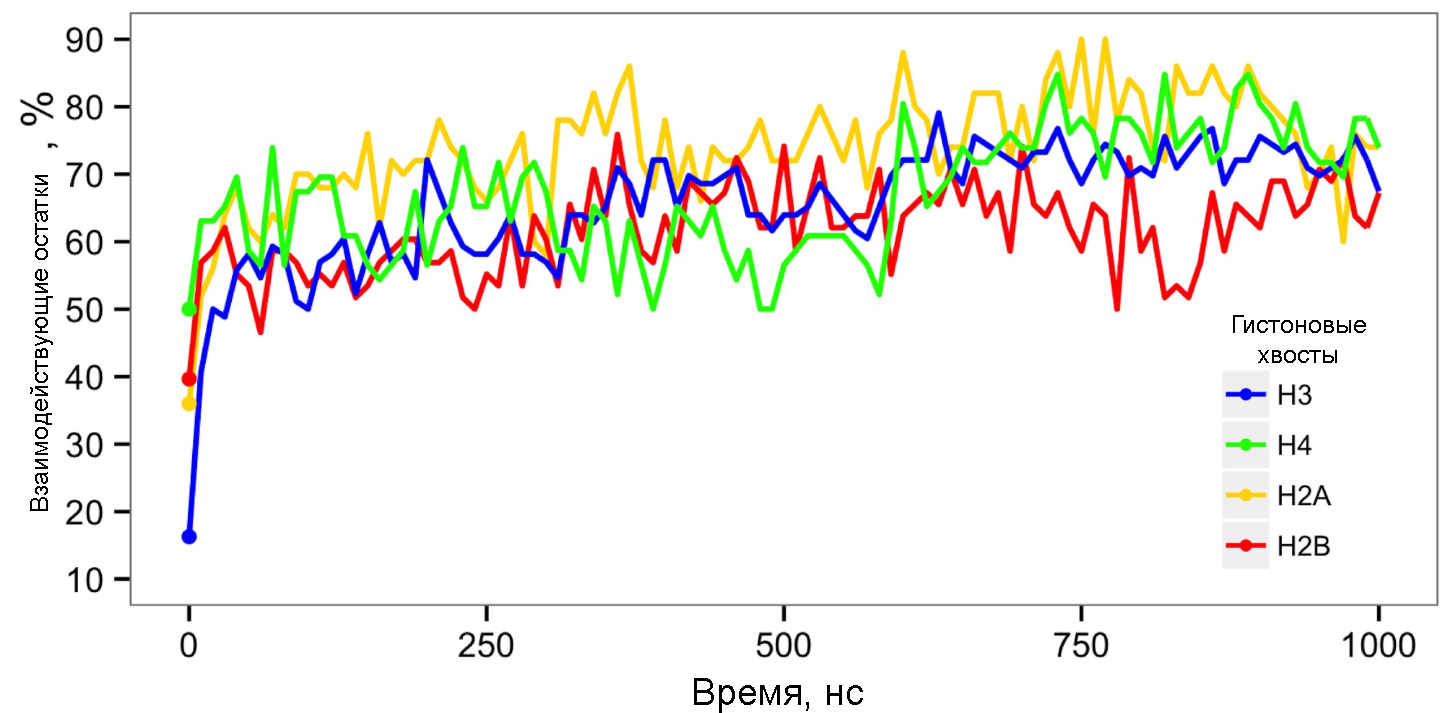
\includegraphics[width=\textwidth]{images/p2/jmb/part2_2_f4.pdf}
    \caption[Конденсация гистоновых хвостов на ДНК]{Конденсация гистоновых хвостов на ДНК. Доля остатков гистонового хвоста, которые имеют прямые или опосредованные водой взаимодействия с ДНК, представлена как функция времени моделирования. Начальные значения обозначены точками.}
    \label{fig:p2_2_f4}
\end{figure}

\begin{figure} [H]
    \centering
    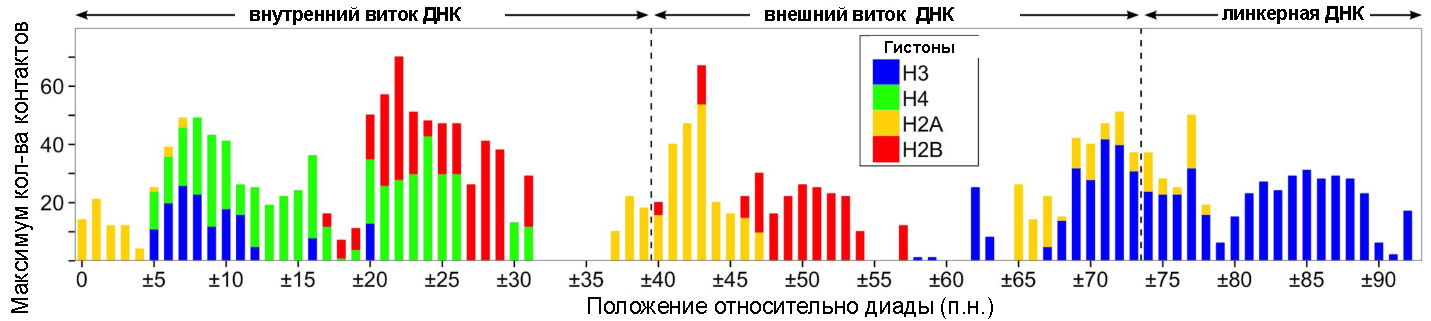
\includegraphics[width=\textwidth]{images/p2/jmb/part2_2_f5.pdf}
    \caption[Доступность ДНК для взаимодействия с гистоновыми хвостами]{Доступность ДНК для взаимодействия с гистоновыми хвостами. Максимальное количество атом-атомных контактов между ДНК и гистоновыми хвостами показано для всех кадров из различных систем моделирования (FN, FNnt и FNbb).}
    \label{fig:p2_2_f5}
\end{figure}



\subsubsection{Хвосты гистонов ``застревают’’ в малых бороздках ДНК и влияют на доступность эпигенетически модифицированных сайтов}
    Конденсация гистоновых хвостов на ДНК в ходе моделирования явно изменила конформационную динамику хвостов и самой ДНК, фактически она напоминала двумерную диффузию на поверхности ДНК с малыми бороздками ДНК, служащими кинетическими ловушками. Несмотря на обширное моделирование, за 1 мкс мы заметили, что хвосты двух копий одного и того же гистона часто исследовали не перекрывающиеся подмножества конформационного пространства. Мы предполагаем, что переключение между различными конформационными подпространствами для таких хвостов происходило во временном масштабе более длительном, чем время нашего моделирования (Рис. \ref{fig:p2_2_f6}). Такое поведение согласуется с экспериментальными данными по химическому  сшиванию и ЯМР гистоновых хвостов \cite{lee_n-terminal_1997,zhou_histone_2012}. Интересно, что в нашем микросекундном моделировании скорость конформационной динамики гистоновых хвостов зависела от их конформации и способа связывания с ДНК. Например, амплитуда колебаний хвоста H3 на одной стороне нуклеосомы, который адсорбируется на линкерной ДНК, была намного выше (из-за гибкости линкерной ДНК) по сравнению с другим хвостом H3, который был компактно свернут на около входа ДНК в нуклеосому. Динамические характеристики гистоновых хвостов в мононуклеосомах и массивах нуклеосом недавно были исследованы с помощью ряда методов, включая твердотельный ЯМР и ЯМР в растворе, дейтеро-водородный обмен \cite{kato_characterization_2009,zhou_histone_2012,gao_histone_2013}. Данные исследования содержат достаточно противоречивые выводы. Принимая во внимание наши результаты, мы предполагаем, что динамика гистоновых хвостов даже в компактных массивах нуклеосом может быть организована неоднородным образом, при этом одни хвосты стабильно свернуты, в то время как другие активно исследуют конформационное пространство.

    Подробный анализ взаимодействий между отдельными боковыми цепями аминокислот и основаниями ДНК указывает на то, что определенные боковые цепи хвостов гистонов могут быть глубоко вставлены в малые бороздки ДНК, взаимодействуя с основаниями ДНК и выступая в качестве якорей, стабилизирующих взаимодействия и ограничивающие конформационную динамику. Наибольшее количество контактов с основаниями ДНК образовано аргининами и лизинами, расположенными внутри гистоновых хвостов. А именно, в основной (FN) модели, следующие остатки показали высокую склонность к взаимодействию с основаниями малой бороздки ДНК: R8 и R26 гистона H3; K16 и R17 гистона H4; R11, K13 и K126 гистона H2A, R29 и R30 гистона H2B. Интересно, что для хвостов H3 и H4 ни одно из этих взаимодействий с основаниями ДНК не наблюдалось в исходной рентгеновской структуре. В то время, как среди контактов белок-ДНК внутри гистонового кора преобладали взаимодействия с фосфатами (в модели FN 82\% - фосфаты, 16\% - сахара, 2\% - основания), в области гистоновых хвостов 17\% контактов - это взаимодействия с основаниями, что значительно больше, чем  количество контактов между основаниями ДНК и гистонами в кристаллической структуре (8\%).

    Следует отметить, что многие упомянутые выше сайты потенциально могут подвергаться посттрансляционным модификациям, включая метилирование аргининов и метилирование и ацетилирование лизинов. Например, два из наиболее важных эпигенетически модифицированных остатков на гистоне H3 (H3K9 и H3K27) расположены рядом с остатками аргинина (H3R8 и H3R26), которые показали высокую тенденцию к встраиванию в малые бороздки ДНК. Следовательно, такие мотивы аргинин-лизин внутри гистоновых хвостов могут влиять на доступность определенных лизинов для эффекторных белков и их способность посттрансляционно модифицироваться.
    
    Если мы проанализируем те сайты, которые устанавливают прямые контакты с нуклеотидами в малой бороздке ДНК в наших моделях, наиболее выраженным является H4K16, который находится в позиции ДНК SHL -1,5. Это хорошо известный сайт ацетилирования, который регулирует компактизацию хроматина и связывание ремоделера ACF \cite{shogren-knaak_histone_2006}. Исследование мононуклеосом методом ЯМР подтвердило гибкость остатков 1-15 хвоста гистона H4, тогда как остатки 16-22 плотно взаимодействуют с нуклеосомным кором и не демонстрируют мобильности в соответствующей шкале времени ЯМР. Более того, было экспериментально подтверждено, что ацетилирование, имитирующее мутацию H4K16Q, которая, согласно нашему исследованию, вероятно, ослабит взаимодействие этого остатка с малой бороздкой ДНК из-за потери положительного заряда боковой цепи, вызывает структурное разупорядочение в этой области \cite{zhou_histone_2012}. В соответствии с нашими наблюдениями, экспериментальное исследование показало, что H4H18 и H4K16 могут быть связаны с позициями ДНК SHL $\pm$1.5 \cite{weng_probing_2014}. Наши наблюдения о связывании малой бороздки с H4K16 также согласуются с более ранними выводами Erler et al. в REMD-моделировании нуклеосом \cite{erler_role_2014}. Совсем недавно Collepardo-Guevara et al. в многомасштабном моделировании показали, что ацетилирование лизина увеличивает содержание вторичных структур в гистоновом хвосте и снижает доступность хвоста для решающих межнуклеосомных взаимодействий, компактизующих хроматиновые волокна \cite{collepardo-guevara_chromatin_2015}, что согласуется с более ранним моделированием конформационного ансамбля фрагментов гистоновых хвостов без ДНК в растворе \cite{potoyan_energy_2011,potoyan_regulation_2012}. Эти результаты также согласуются с более ранней работой по моделированию взаимодействий ДНК с пептидами из H4-хвоста \cite{korolev_h4_2007,korolev_molecular_2014}, в которой авторы предположили, что заряженные группы аргининов и лизинов играют главную роль в притяжении ДНК-ДНК через хвост гистона, образуя мосты между фосфатными группами и взаимодействую с электроотрицательными участками в малой бороздке.

    Наш сравнительный анализ взаимодействий гистонов с ДНК в различных областях нуклеосомы предполагает, что большинство взаимодействий в области глобулярных частей гистонов обеспечивается преимущественно остатками аргинина, в то время как взаимодействия между хвостами гистонов и ДНК почти в равной степени обеспечиваются остатками аргинина и лизина (Рис. \ref{fig:p2_2_f7}). Это не относится к исходной конформации, происходящей из кристаллической структуры NCP, где взаимодействия белок-ДНК через остатки лизина в значительной степени недостаточно представлены. Хотя следует отметить, что в кристаллической структуре NCP дополнительные контакты гистон-ДНК могут формироваться с соседними нуклеосомами в кристаллической решетке, которые мы не включаем в наш анализ. Такая тенденция согласуется со склонностью аргининов находится в малых бороздках ДНК, как это наблюдалось в кристаллических структурах многих комплексов белок-ДНК \cite{rohs_role_2009}. Как видно из рисунка \ref{fig:p2_2_f7}, глицин также преобладает в H3, H2A и особенно в N-концевых хвостах H4, и его карбонильная группа основной цепи может образовывать неспецифические контакты с фосфатами основной цепи ДНК. Важно отметить, что, хотя прямые контакты белков с основаниями ДНК (прямое считывание) обычно считаются почти отсутствующими в нуклеосомах и не влияют на позиционирование нуклеосом, это может быть слишком упрощенной картиной. Например, было показано, что гистоновые хвосты могут вносить вклад в зависимое от последовательности позиционирование нуклеосом \cite{yang_core_2007}. Однако этот эффект не воспроизводился на последовательностях с высоким сродством. Обширные контакты гистоновых хвостов с основаниями ДНК, наблюдаемые в нашем исследовании, могут помочь понять и интерпретировать эти экспериментальные результаты.

\subsubsection{Выпячивание ДНК возле точек входа/выхода модулируется конформациями гистонового хвоста}
    Теперь обратим внимание на анализ связи между конформацией гистоновых хвостов и геометрией нуклеосомной ДНК. В ходе моделирования проявились некоторые изменения в конформации ДНК (Рис. \ref{fig:p2_2_f3}aб). Самая большая замеченная перестройка -- выпячивание ДНК рядом с ее точкой входа в нуклеосому в районе SHL $\pm$6,5. Данную перестройку можно было наблюдать только во временных масштабах более 100 нс, и она была обусловлена различными конформациями гистоновых хвостов (Рисунок \ref{fig:p2_2_f6}). Взаимодействия в этой области ДНК (концевые 10 п.н. коровой ДНК) в основном представлены взаимодействиями с гистоновыми хвостами, а не с глобулярными доменами, что позволяет предположить, что гистоновые хвосты могут оказывать сильное влияние на конформацию ДНК, приводя к потенциальной стабилизации или дестабилизации всей нуклеосомы. Действительно, в моделировании FN-модели терминальная коровая область ДНК вокруг SHL +6,5 образовывала намного больше контактов с гистоновыми хвостами, чем ее симметричный аналог в SHL -6,5 (184 контакта против 64), что вызывало ее стабилизацию и предотвращало выпячивание ДНК. Эта стабилизация, по-видимому, была вызвана обширными взаимодействиями с N-концевым хвостом H3, который формирует компактную вторичную структуру около места входа / выхода ДНК, а также вставкой H2A K126 в малую бороздку ДНК (Рис. \ref{fig:p2_2_f6}). Таким образом С-концевой хвост H2A также может участвовать в стабилизации ДНК. Фактически, недавно было экспериментально обнаружено, что частичная делеция С-концевой области H2A приводит к разворачиванию последних 10 п.н. коровой ДНК \cite{shukla_docking_2011}. В соответствии с этим фактом, колебания концевых частей коровой ДНК были менее ограниченными в нашем моделировании для системы NCPm, которая имела усеченные гистоновые хвосты (Рис. \ref{fig:p2_2_f3}aб).


\begin{figure} [H]
    \centering
    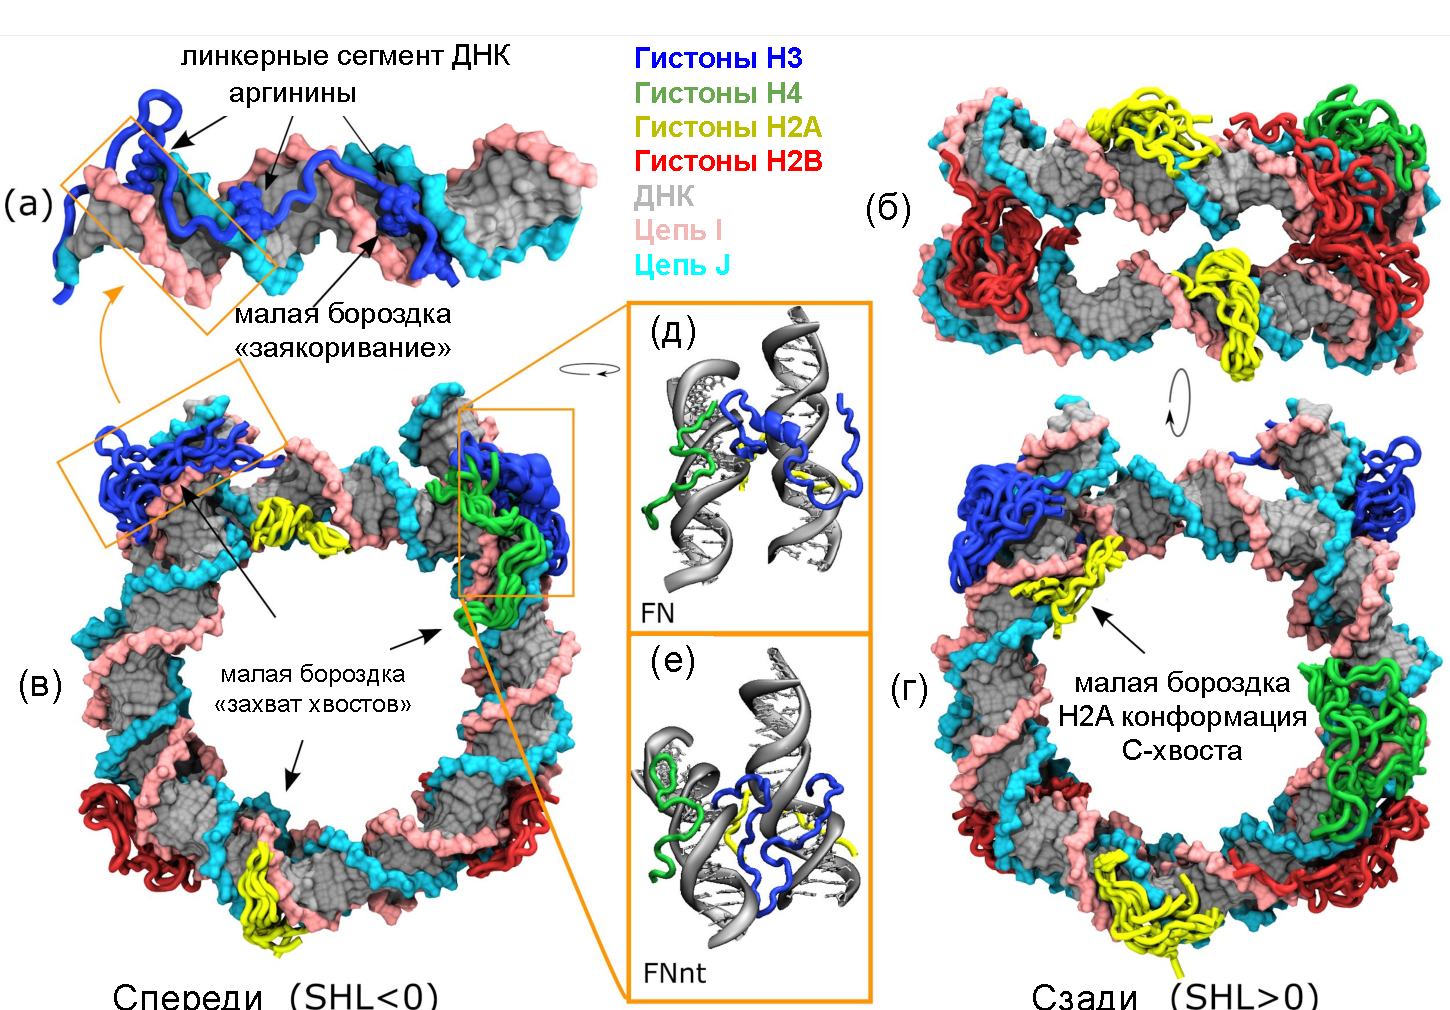
\includegraphics[width=\textwidth]{images/p2/jmb/part2_2_f6.pdf}
    \caption[Типичные паттерны взаимодействия гистоновых хвостов с ДНК]{Типичные паттерны взаимодействия гистоновых хвостов с ДНК, наблюдаемые при МД моделировании. (а) Типичная конформация N-концевого хвоста H3, взаимодействующего с линкерной ДНК. (б) - снизу, (в) - спереди и (г) - виды нуклеосомы с множественными наложенными конформациями гистонового хвоста, наблюдаемыми в течение 1 мкс МД моделирования (изображены каждые 100 нс с отброшенными первыми кадрами 250 нс). (д) формирование $\alpha$-спирали, образованной остатками 21-28 одного из хвостов H3 (цепь A), (е) альтернативное стабильное положение хвоста H3, ``состыкованное'' между супервитками ДНК.}
    \label{fig:p2_2_f6}
\end{figure}

\begin{figure} [H]
    \centering
    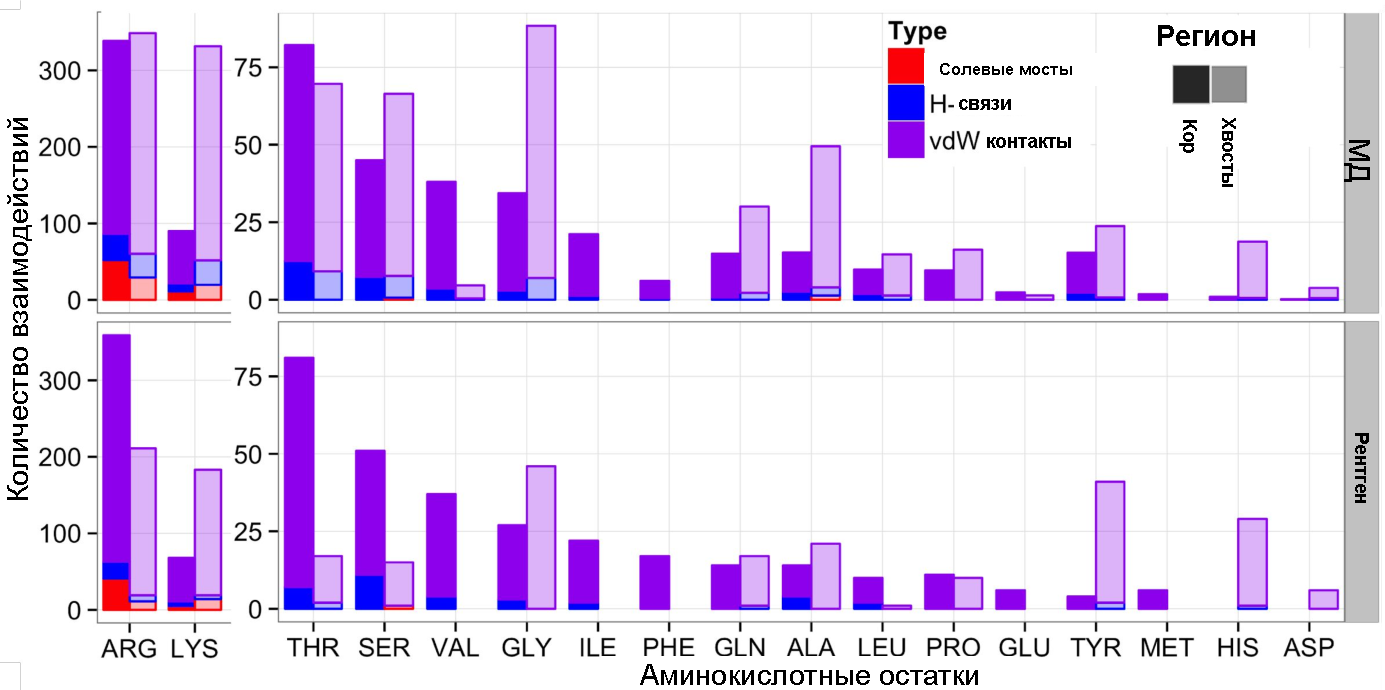
\includegraphics[width=\textwidth]{images/p2/jmb/part2_2_f7.pdf}
    \caption[Взаимодействия белок-ДНК в нуклеосоме]{Количественная оценка взаимодействий белок-ДНК по типу, участку гистона и участвующим аминокислотам.}
    \label{fig:p2_2_f7}
\end{figure}

\begin{figure} [H]
    \centering
    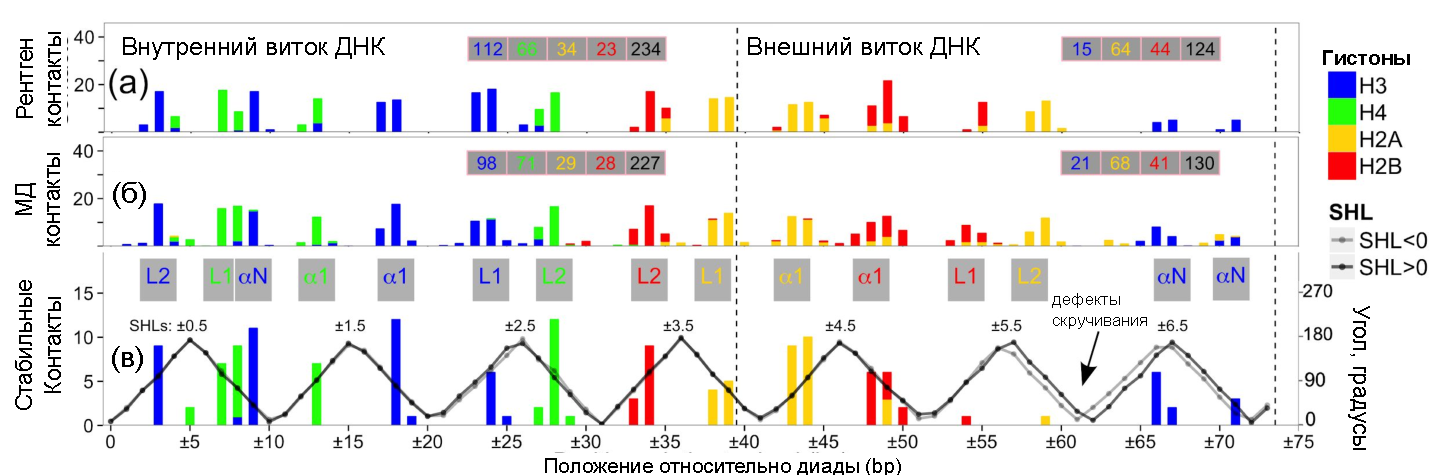
\includegraphics[width=\textwidth]{images/p2/jmb/part2_2_f8.pdf}
    \caption[Взаимодействия белок-ДНК в области нуклеосомного кора]{Взаимодействия белок-ДНК в области нуклеосомного кора. (а) Профиль контактов для рентгеновской структуры, усредненный по двум половинам нуклеосомы. (б) Среднее количество контактов по всем кадрам и по симметричным половинам нуклеосомы. Общее количество контактов для соответствующих участков ДНК и гистонов показано в розовых рамках для графиков (а) и (б). (в) Количество стабильных контактов белок-ДНК. В каждой позиции ДНК указывается количество уникальных стабильных контактов атом-атом, наблюдаемых на любой половине нуклеосомы (т.е. связанные с симметрией стабильные контакты, наблюдаемые в двух половинах нуклеосомы, подсчитывались только один раз, асимметричные контакты вносились индивидуально). Структурные элементы сайтов связывания ДНК аннотированы в верхней части этого графика разными цветами, соответствующими разным типам гистонов. Черные и серые кривые показывают периодичность вращения ДНК в структуре нуклеосом, усредненной по траектории.}
    \label{fig:p2_2_f8}
\end{figure}





\subsubsection{Сайты связывания ДНК в гистоновом коре демонстрируют возможность перестройки, сопровождающейся образованием дефектов кручения ДНК}
    В наших предыдущих разделах мы говорили о взаимодействиях между гистоновыми хвостами и ДНК; в этом разделе мы обсудим взаимодействия гистонов с ДНК, вовлекающие глобулярные домены гистонов, и их связь с перестройками геометрии ДНК. Из анализа кристаллической структуры NCP известно, что ДНК имеет семь пар симметричных сайтов связывания, где малая бороздка ДНК обращена к октамеру гистонов. В каждом сайте связывания ключевой аргинин вставлен в малую бороздку в большинстве случаев, за исключением канонических аргининов R49 из обеих копий H3, которые расположены слишком далеко, чтобы их можно было вставить в малую бороздку в районе SHL $\pm$6.5. В то же время это место имеет небольшое количество контактов с гистоновым ядром (Рис. \ref{fig:p2_2_f8}а,б). Наш анализ динамики взаимодействий гистон-ДНК показал, что этот канонический H3R49 действительно может быть вставлен в соответствующую малую бороздку из-за выпячивания ДНК в районе SHL $\pm$6.5, описанной ранее. Этому выпячиванию, по-видимому, способствовало образование дополнительных и перестройка существующих контактов между $\alpha$N-спиралью H3 и ДНК. Чтобы понять последствия этих изменений для общей геометрии ДНК, мы построили график эффективного вращения пар оснований ДНК относительно положения суперспиральной оси (Рис. \ref{fig:p2_2_f8}в). Мы наблюдали сдвиг в общем скручивании ДНК на одну пару оснований вокруг SHL -6/-6,5, а в случае модели NCPm такие сдвиги наблюдались в области от SHL -5,5 до конца коровой ДНК. Подобные сдвиги в геометрии скручивания ДНК ранее были названы ``твист-дефектами'' \cite{edayathumangalam_nucleosomes_2005}. Некоторые экспериментальные исследования показали, что нуклеосома существует в растворе как смесь различных состояний твист-дефектов, и только некоторые из них могут быть увидены в кристаллических структурах путем изменения основной последовательности ДНК, ее длины или добавления интеркалирующих агентов \cite{edayathumangalam_nucleosomes_2005}. В нашем исследовании мы впервые смогли наблюдать образование таких дефектов \textit{in silico} и описать атомистические детали, лежащие в основе связи между геометрией ДНК и взаимодействиями гистон-ДНК.
    
    Чтобы выяснить закономерности взаимодействий в различных сайтах связывания гистонов с ДНК, мы вычислили количество так называемых стабильных контактов (см. Методы). Как видно на рисунках \ref{fig:p2_2_f8}a-в, количество контактов между гистоновым кором и внутренним супервитком ДНК было почти вдвое больше, чем количество контактов с внешним витком ДНК. Это согласуется с более легким разворачиванием внешнего витка ДНК в экспериментах с единичными молекулами \cite{hall_high_2009,brower-toland_mechanical_2002}. Более того, рисунок \ref{fig:p2_2_f8} показывает четкую иерархию между различными каноническими сайтами связывания. Сайты связывания вокруг SHL $\pm$0,5 и SHL $\pm$4,5 имеют наибольшее количество динамически стабильных контактов в соответствии с картированием с высоким разрешением взаимодействий белок-ДНК в нуклеосомах, полученным путем механического растягивания ДНК. Последние эксперименты показали, что наиболее сильные взаимодействия гистон-ДНК происходят вокруг диады и в районе расположения $\pm$40 пар оснований от диады \cite{hall_high_2009}.
    
    Первый сайт связывания гистонов с ДНК вокруг SHL $\pm$0,5 образован петлями L1/L2 димера H3-H4, с дополнительным взаимодействием, исходящим от N-конца $\alpha$N-спирали H3, что делает этот сайт очень особенным с точки зрения его уникальной специфической организации. Различия между паттернами связывания гистонов с ДНК наблюдались на картах нуклеосом по всему геному, и недавно с помощью геномного анализа позиционирования нуклеосом был обнаружен необычный сигнал относительно содержания A|T/G|C в нуклеосомной ДНК в девяти парах оснований от центра нуклеосомы \cite{brogaard_map_2012}. Предполагалось, что это может быть связано с внедрением H3R40 глубоко в малую бороздку ДНК, либо с образованием специфичных для последовательности контактов с основаниями \cite{davey_does_2013}. Однако мы не наблюдали таких контактов в микросекундном масштабе времени, и H3R40 взаимодействовал с фосфатами ДНК, а не с основаниями.
    
    Второй высокостабильный сайт связывания вокруг SHL $\pm$4.5 образован двумя $\alpha$1-спиралями димера H2A-H2B, тогда как сайты связывания ДНК с наименьшим числом стабильных взаимодействий локализованы на SHL $\pm$6.5, SHL $\pm$5.5 и SHL $\pm$1.5. Карта контактов гистонов с ДНК согласуется с профилем флуктуаций ДНК (Рис. \ref{fig:p2_2_f9}), а флуктуации ДНК показывают видимое увеличение при SHL $\pm$1,5. Это согласуется с повышенной конформационной гибкостью ДНК в этих сайтах при связывании малых молекул или белков показанной в недавних экспериментах. Эти эксперименты показали, что SHL $\pm$1,5 является местом связывания ионов тяжелых металлов и интеркалирующих противоопухолевых агентов \cite{tan_nucleosome_2011}. Отсутствие стабильных взаимодействий вокруг SHL $\pm$5.5/$\pm$6.5 также соответствует увеличению флуктуаций ДНК. Колебания на самом конце коровой ДНК несколько меньше, что объясняется их стабилизацией через N- и С-концевые хвосты H3 (см. Предыдущие разделы). Малая стабильность и высокая гибкость сайтов связывания SHL $\pm$5.5 и SHL $\pm$6.5 может указывать на то, что эти сайты вносят лишь небольшие энергетические барьеры при разворачивании ДНК из нуклеосомы. Биологически значимый процесс, который основан на таком постепенном разрыве контактов ДНК-гистонов, включает транскрипцию РНК-полимеразами, которая может происходить без вытеснения нуклеосом \cite{studitsky_mechanism_1997}. Нуклеосомный барьер для транскрипции, исследованный с помощью паттернов транскрипционного паузирования, показал, что первый барьер встречается полимеразой, когда передний край полимеразы входит в область примерно в 40 п.н. от диады \cite{jin_synergistic_2010}. Данный факт согласуется с представлением о том, что первые два сайта связывания почти не представляют барьера для транскрипции.


\begin{figure} [H]
    \centering
    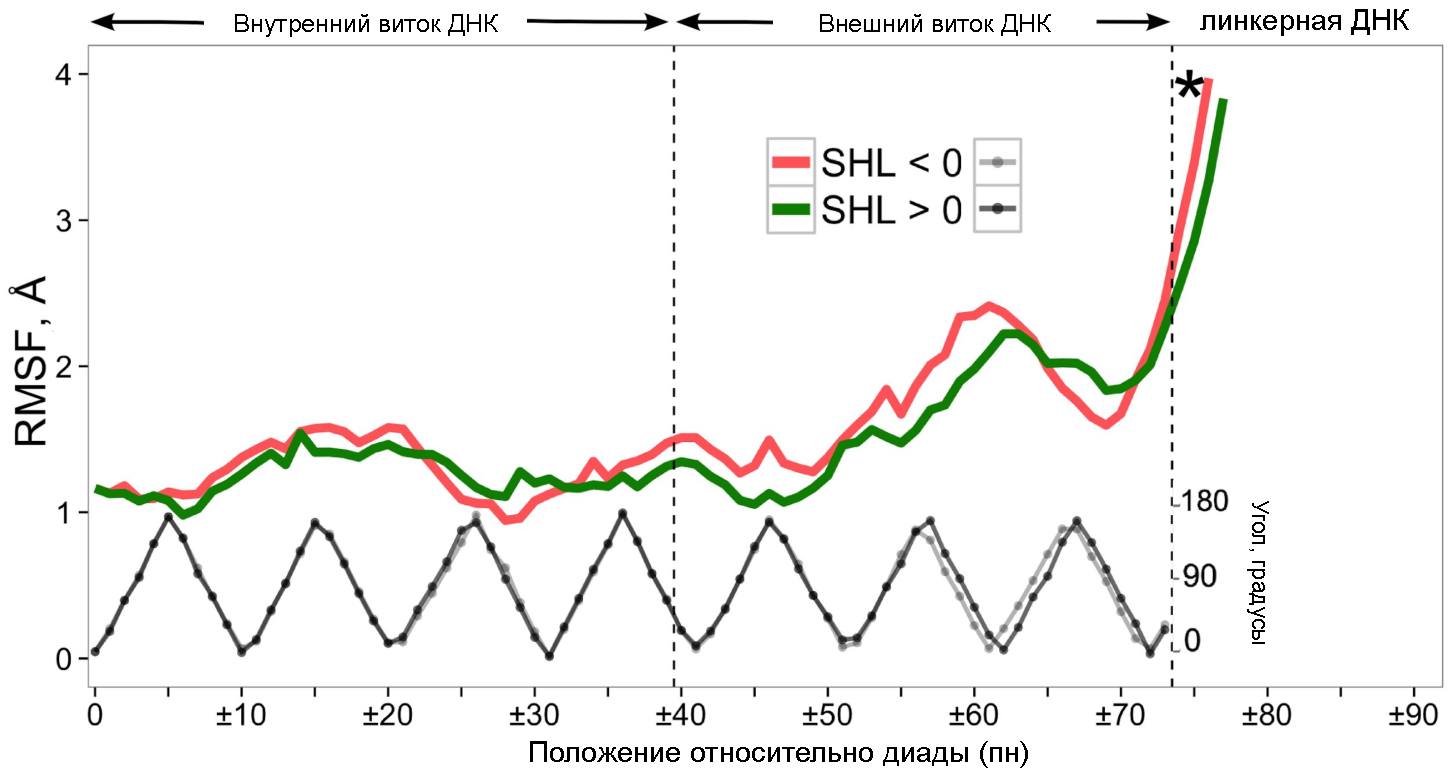
\includegraphics[width=\textwidth]{images/p2/jmb/part2_2_f9.pdf}
    \caption[Флуктуации ДНК в нуклеосоме]{Флуктуации ДНК в нуклеосоме. RMSF центров пар оснований для двух симметричных половин нуклеосом (красная и зеленая кривые); черные и серые кривые показывают периодичность вращения суперспирали ДНК. Точки данных, превышающие RMSF 4\AA, не показаны. Звездочкой обозначена та же цепь, что и на рисунке \ref{fig:p2_2_f3}.}
    \label{fig:p2_2_f9}
\end{figure}

\subsection{Обсуждение}
    В данном разделе мы представили молекулярно-динамическое исследование полной модели нуклеосомы с полноразмерными гистоновыми хвостами и линкерными участками ДНК. Мы использовали полноатомное моделирование в явном растворителе и распространили этот подход на микросекундную шкалу времени. Микросекундная шкала времени и многочисленные сравнительные симуляции позволили нам получить представление о функционально значимых перестройках в конформациях нуклеосом, включая связь между конформациями гистоновых хвостов и ДНК.

    Механистические наблюдения, полученные в нашем исследовании, предполагают, что конформационные перестройки внутри коровой ДНК зависят от паттернов взаимодействий ДНК с гистонами. В частности, мы наблюдали, что N-концевой хвост H3 и C-концевой хвост H2A устанавливают много контактов с коровой ДНК и могут стабилизировать геометрию ее концевой области, подавляя образование локализованных дефектов кручения внутри ДНК. С другой стороны, конформация хвостов, которые выступают из нуклеосомы, способствуют образованию состояний с дефектами кручения, которые могут быть важными промежуточными звеньями в скольжении и ремоделировании нуклеосом \cite{mueller-planitz_nucleosome_2013}. Мы предлагаем наличие механизма, с помощью которого наблюдаемое чрезмерное скручивание ДНК в терминальной области ДНК может представлять собой начальное состояние дефекта кручения ДНК, которое может быть стабилизировано последующими перестройками взаимодействий ДНК в центральной области гистонов. Последующее скольжение нуклеосом может происходить за счет распространения этого дефекта дальше по кору нуклеосомы. Интересно отметить, что несколько исследований по химическому сшиванию мононуклеосом \textit{in vitro} ранее показали, что гистоновые хвосты занимают различные предпочтительные конформации в NCP, нуклеосомах с линкерами и нуклеосомами с гистоном H1 \cite{lee_linker_1998,angelov_preferential_2001}. Данный факт позволяет предположить, что гистоновые хвосты очень чувствительны к наличию/отсутствию линкерной ДНК, гистона H1 и изменений в нуклеосомном окружении.
    
    В соответствии с результатами экспериментов по химическому сшиванию  ДНК с гистонами \cite{angelov_preferential_2001,stefanovsky_laser-induced_1989} мы обнаружили, что гистоновые хвосты легко адсорбируются на линкерную (в основном хвосты H3) и коровую ДНК (в основном хвосты H4, H2B и H2A), и большинство контактов гистонов с ДНК представлено контактами с гистоновыми хвостами. О возможности взаимодействия N-концевых хвостов H3 с линкерной ДНК сообщалось ранее \cite{rhee_subnucleosomal_2014,angelov_preferential_2001}. Фактически, эффективность химического сшивания в NCP оказалась в 3–4 раза ниже для H2A, H2B и H4 и в 10–12 раз ниже для H3 по сравнению с полными нуклеосомами с линкерной ДНК \cite{stefanovsky_laser-induced_1989}. Более того, наше детальное изучение поведения гистоновых хвостов показало, что их динамика в микросекундном масштабе характеризуется ограниченной диффузией на поверхности ДНК и кинетическим захватом хвостовых областей в малых бороздках ДНК. Наблюдаемое стабильное прикрепление гистоновых хвостов к коровой и линкерной ДНК предполагает глубокие последствия для взаимодействий нуклеосом с другими белками хроматина. В самом деле, когда эти белки связываются с гистоновыми хвостами или ДНК, сначала они должны проконкурировать со взаимодействиями ДНК-гистоновый хвост и вытеснить соответствующего партнера. Например, Pilotto et al. недавно экспериментально продемонстрировали элегантную практическую иллюстрацию этой концепции на примере комплекса LSD1-CoREST, который действует как деметилаза H3K4 \cite{pilotto_interplay_2015}. Было высказано предположение, что этот комплекс связывается с нуклеосомой через свою субъединицу CoREST, которая вытесняет хвост H3 с ДНК. Это смещение критически необходимо для того, чтобы сделать метилированный H3K4 доступным для взаимодействий с его субъединицей LSD1. Можно предположить, что такие механизмы могут быть использованы для организации перекрестного взаимодействия между множественными сайтами связывания на гистоновых хвостах, включая сайты ПТМ и их соответствующих партнеров по связыванию \cite{ruthenburg_multivalent_2007,nishi_crosstalk_2015}.
    
    Атомистические детали связывания гистонового хвоста с ДНК, выявленные в ходе нашего исследования, дополнительно показали, что этому процессу способствует вставка закрепляющих боковых цепей аргинина и лизина в малые бороздки ДНК. Это, в свою очередь, повлияло на те остатки, которые служат эпигенетически модифицированными сайтами в хвостах гистонов, или на остатки, расположенные рядом с ними (например, H3K9, H3K27, H4K16 и H3R8, H3R26 и т.д.). Присутствие множества сайтов связывания на одном хвосте гистонов и окклюзия боковой цепи малыми бороздками может вызывать кооперативные эффекты. А именно, связывание одного партнера с его сайтом связывания на ДНК или сайтом гистонового хвоста может вызвать смещение гистонового хвоста от ДНК и, таким образом, облегчать связывание другого партнера. Подобные эффекты могут быть вызваны посттрансляционными модификациями, такими как метилирование аргинина и особенно ацетилирование лизина, которые не способствуют встраиванию этих остатков в малую бороздку и, таким образом, могут способствовать конформационной гибкости и доступности связывания гистоновых хвостов. Наблюдаемые эффекты помогают наметить дальнейший план экспериментальных исследований, которые должны прояснить сложное динамическое взаимодействие между посттрансляционными модификациями гистонов и доступностью гистоновых хвостов для связывания эффекторных белков.

\subsection{Материалы и методы}
\subsubsection{Построение начальной модели}
    В качестве отправной точки мы использовали рентгеновскую кристаллическую структуру высокого разрешения (1,9\AA) коровой частицы нуклеосомы, образованную рекомбинантными вариантами канонических коровых гистонов \textit{X. laevis}и модифицированной $\alpha$-сателлитной ДНК человека (PDB ID 1KX5 \cite{davey_solvent_2002}). Для создания полной нуклеосомной модели с линкерными сегментами ДНК с помощью программы NAB был сконструирован прямой дуплекс B-ДНК $(AGTC)_5$ длиной 20 п.н. \cite{macke_thomas_modeling_1997}. Используемая линкерная последовательность ДНК сбалансирована по количеству гибких и жестких динуклеотидов \cite{olson_dna_1998}. Она была прикреплена к основной ДНК на обоих концах NCP. Один из хвостов гистона H3 был слегка повернут, чтобы избежать стерических столкновений с линкерной ДНК (угол $\Psi$ Lys36 был установлен на -35 градусов) (Рис. \ref{fig:p2_2_f1}a). Минималистичная модель NCP (NCPm) была получена из той же кристаллической структуры путем усечения гистоновых хвостов в сайтах, указанных на рисунке \ref{fig:p2_2_f2} треугольниками. Все модели были явно сольватированы в прямоугольной ячейке с минимальным расстоянием между растворенным веществом и границами ячейки в 20\AA, за исключением системы FNbb (таблица 1), для которой использовался порог в 100\AA. В системы добавляли ионы натрия для нейтрализации, а затем добавляли дополнительные ионы натрия и хлора в концентрации 150 мМ по отношению к объему воды, за исключением системы FN1M, где использовалась концентрация 1 М. Точная соответствующая объемная концентрация ионов была оценена непосредственно из данных моделирования. Кристаллографические молекулы воды остались в системе, а все кристаллографические ионы были удалены. Состояния протонирования аминокислот определяли на основании значений pK их растворов при нейтральном pH, остатки гистидина считали нейтральными и протонировали на $\epsilon$-азотах. Модель FNnt была идентична модели FN, но имела нейтрально заряженные белковые концы для изучения устойчивости МД-моделирования к небольшим возмущениям. Структуры исходных моделей представлены на рис. \ref{fig:p2_2_f1}а. На выбор NaCl в качестве соли для нашего моделирования повлияло его обычное использование в экспериментах с нуклеосомами \textit{in vitro}, а также в протоколах сборки нуклеосом \cite{dyer_reconstitution_2004}.

\subsubsection{Протоколы моделирования и выбор силового поля}
    Силовое поле CHARMM36 использовалось для ДНК и белка \cite{best_optimization_2012,hart_optimization_2012}, параметры TIP3P для молекул воды и скорректированные параметры  Луо и Ру для ионов \cite{luo_simulation_2010}. Выбор силового поля всегда является деликатным вопросом из-за известных и неизвестных приближений, используемых в силовом поле, а также постоянными усилиями по улучшению силового поля, предпринимаемых разработчиками. В случае нуклеосом проблема осложняется необходимостью сочетать точные модели белков и ДНК, а также обеспечивать реалистичное моделирование взаимодействий с растворителем. Ниже мы кратко обсудим несколько недавних современных исследований о поведении различных силовых полей при моделировании нуклеосом.
    
    Точность силового поля белка, по-видимому, особенно важна для моделирования поведения изначально неупорядоченных гистоновых хвостов. Систематические исследования биомолекулярных силовых полей \cite{lindorff-larsen_systematic_2012} показали, что определенные силовые поля (например, CHARMM27, AMBER ff03) сверхстабилизируют спиральную конформацию пептидов, и поэтому эта проблема была решена в пересмотре силового поля для белков CHARMM36 \cite{best_optimization_2012}. Кроме того, несколько недавних исследований поставили под сомнение применимость силовых полей белков для специфического моделирования гистоновых хвостов \cite{erler_role_2014,collepardo-guevara_chromatin_2015,potoyan_energy_2011}. Например, Erler et al. показали, что разные версии силовых полей AMBER могут приводить к разному динамическому поведению гистоновых хвостов \cite{erler_role_2014}. Collepardo-Guevara et al. сравнили результаты моделирования с использованием современных силовых полей, включая CHARMM36, с данными ЯМР по динамике гистонового хвоста и пришли к выводу, что все силовые поля дают почти идентичные результаты \cite{collepardo-guevara_chromatin_2015}.

    Силовое поле ДНК необходимо для правильного воспроизведения конформационных переходов ДНК при моделировании нуклеосом. Параметризация силовых полей нуклеиновых кислот оказывается более сложной задачей, чем аналогичная задача для белков. В настоящее время известно, что силовые поля как CHARMM, так и AMBER воспроизводят стабильную динамику ДНК в микросекундном масштабе времени и за его пределами \cite{galindo-murillo_convergence_2015}. Однако точное воспроизведение экспериментальных результатов по зависимой  деформируемости ДНК от последовательности с использованием доступных силовых полей все еще остается нерешенной проблемой \cite{perez_frontiers_2012}.
    
    Наши модельные системы были подготовлены с помощью программы VMD \cite{humphrey_vmd_1996}, а моделирование МД было выполнено с помощью пакета NAMD 2.9 \cite{phillips_scalable_2005}. Для моделирования при постоянной температуре использовался подход динамики Ланжевена с шагом интегрирования 2 фс, параметром демпфирования 0,5 $пс^{-1}$ и T = 310K. Поддержание давления в 1 атм было реализовано методом Ланжевена. Моделирование проводилось с жесткими ковалентными связями, и ван-дер-ваальсовы взаимодействия постепенно выключались на расстоянии от 10 до 12\AA. В электростатических расчетах использовался метод PME с шагом сетки 1\AA, кубической интерполяцией, отсечкой в реальном пространстве 12\AA и параметром толерантности $10^{-6}$. Использовались периодические граничные условия. Для устранения диффузии нуклеосом к атомам C-$\alpha$ гистоновых фолдов H3 (номера остатков 64-78, 86-114, 121-131) применялись небольшие позиционные ограничения в 0,003 ккал/моль/$A^2$. Чтобы избежать расплетания пар оснований на концах ДНК в моделировании NCPm, использовали ограничивающий потенциал в виде искусственной стенки, чтобы сохранить расстояние между центрами масс оснований в концевых парах оснований в пределах 120\% от начального.

    Все системы были подвергнуты минимизации энергии и первоначальному уравновешиванию. Затем проводилось моделирование до времени моделирования 1 $\mu$с. Кадры траектории сохранялись каждые 100 пс. Мы запускали расчеты параллельно на высокопроизводительных компьютерных кластерах/суперкомпьютерах, используя эффективное распараллеливание, доступное в NAMD. Скорость моделирования варьировалась в зависимости от моделируемой системы, количества процессоров и архитектуры машины. Для справки: система модели FN моделировалась параллельно на 384 ядрах ЦП в течение 120 дней со скоростью $\sim$8 нс/день.
%21 страница

\subsubsection{Анализ траекторий}
    Анализ и визуализация траектории выполнялись с использованием набора библиотек и скриптов собственной разработки, написанных на TCL, Python и R, которые использовали возможности VMD \cite{humphrey_vmd_1996} и 3DNA \cite{lu_3dna_2008} для общего и специфического анализа структуры ДНК. Для структурного анализа нуклеосом отдельные кадры траектории были наложены на исходную кристаллическую структуру, путем минимизации значения среднеквадратичного отклонения (RMSD) между положениями атомов C-$\alpha$ спиралей гистоновых фолдов. Анализ конформации ДНК проводили по отношению к нуклеосомной суперспиральной системе отсчета, определяемой ее диадной осью и суперспиральной осью. Периодичность вращения ДНК в нуклеосоме определяли путем расчета угла между вектором пары оснований (соединяющим атомы N1 и N9 соседних оснований в паре оснований) и суперспиральной осью нуклеосомы. Максимумы и минимумы значений периодичности вращения соответствовали целочисленным и полуцелым значениям SHL.
    
    Подробный анализ взаимодействий гистонов с ДНК проводился для каждого кадра траектории (первые кадры 250 нс не учитывались как начальный период конформационного уравновешивания) путем анализа положений соответствующих атомов. Контакты (SC) между двумя атомами гистона и ДНК определялись как контакты между тяжелыми атомами на расстоянии менее 3,9\AA. Контакты были дополнительно классифицированы следующим образом: солевые мостики (SB) включают два заряженных неводородных атома на расстоянии менее 3,9\AA; водородные связи (HB) были определены как связи между донорными (D) и акцепторными (A) атомами с водородом между ними (DH-A), где расстояние между D и A было меньше 3,5\AA, а DH-A угол составлял больше 150 градусов; контакты Ван-дер-Ваальса (vdW) были определены как контакты между атомами, которые не были связаны водородными связями и не образовывали солевой мостик; и опосредованные водой взаимодействия (WM) определялись как взаимодействия между неводородными атомами ДНК или гистонами, которые образуют водородную связь с одной и той же молекулой воды. Мы также ввели понятие стабильных контактов между ДНК и белком, чтобы описать контакты, которые сохранялись во время моделирования. А именно, они были определены как отдельные пары атомных контактов между ДНК и молекулами белка, которые присутствовали более чем в 80\% кадров траектории после начального периода конформационного уравновешивания.

\subsubsection{Соглашения об описании структуры нуклеосом}
    Позиции пар оснований ДНК были пронумерованы относительно центральной пары оснований (называемой диадой), ее положение принималось равным нулю. Вращательная ориентация двойной спирали ДНК полуколичественно описывается параметром сверхспирального расположения (SHL) (Рис. \ref{fig:p2_2_f1}a), который мы расширяем, чтобы включить не только коровую ДНК (SHL от 0 до $\pm$7), но и линкерную ДНК (SHL до $\pm$9). Исходные 147 пар оснований ДНК NCP называются ``коровой ДНК'', а области, где коровая ДНК соединяется с линкерной ДНК, называются сайтами входа/выхода ДНК. Мы различаем две части в каждом гистоне: область хвоста (как указано на рисунке \ref{fig:p2_2_f2}) и остальную часть, называемую глобулярной частью гистона. Ключевыми элементами глобулярных областей являются спирали гистоновых фолдов $\alpha$1, $\alpha$2 и $\alpha$3 \cite{baxevanis_variety_1995} и петли L1, L2, как показано на рисунке \ref{fig:p2_2_f2}.


\subsubsection{Благодарности}
Исследования данного раздела были поддержаны программами внутренних исследований Национальной медицинской библиотеки и Национального института рака, Национальных институтов здоровья; и Российским научным фондом [грант № 14-24-00031] (разработка алгоритмов визуализации нуклеосом). Автор был поддержан программой сотрудничества между США и Россией в области биомедицинских наук. В этом исследовании использовались высокопроизводительные вычислительные возможности кластера Biowulf Linux в Национальном институте здравоохранения, Бетесда, Мэриленд \url{http://biowulf.nih.gov}. Данное исследование было частично поддержано Суперкомпьютерным центром МГУ им. М.В. Ломоносова и вычислительными ресурсами суперкомпьютера Hexagon Cray XE6m-200, в университете Бергена и норвежском метацентре высокопроизводительных вычислений (NOTUR).








